 	%Install required packages (AMS-LaTeX, natbib, textcase, and bm)

\documentclass[aps,pra,reprint,superscriptaddress]{revtex4-1}
%,nofootinbib
\usepackage{graphicx}
\usepackage{fullpage}
\usepackage{upgreek}
\usepackage{verbatim}
\usepackage{graphicx,epstopdf}
\usepackage{xcolor}
\usepackage{braket}
\usepackage{soul}
%\usepackage{gensymb}

\bibliographystyle{apsrev4-1}

\begin{document}


\title{Imaging small numbers of {\color{gray}(single?)} Ba atoms in solid xenon for barium tagging in nEXO} 

%putting \newline in next to J Albert makes the linew break, but then makes us start at left, uncentered ...
%\author{\hspace{30mm} T.~Walton}
\author{T.~Walton}
\affiliation{Physics Department, Colorado State University, Fort Collins CO, USA}
\author{C.~Chambers}
\affiliation{Physics Department, Colorado State University, Fort Collins CO, USA}
\author{A.~Craycraft}
\affiliation{Physics Department, Colorado State University, Fort Collins CO, USA}
\author{W.~Fairbank Jr.}\thanks{Corresponding author}
\affiliation{Physics Department, Colorado State University, Fort Collins CO, USA}
%\author{\newline \newline J.B.~Albert}
%\author{\newline J.B.~Albert}
\author{J.B.~Albert}
\affiliation{Physics~Department~and~CEEM,~Indiana~University,~Bloomington~IN,~USA}
\author{D.J.~Auty}
\affiliation{Department of Physics and Astronomy, University of Alabama, Tuscaloosa AL, USA}
\author{P.S.~Barbeau}
\affiliation{Department of Physics, Duke University, and Triangle Universities Nuclear Laboratory (TUNL), Durham North Carolina, USA}
\author{ V. ~Basque}
\affiliation{Physics Department, Carleton University, Ottawa ON, Canada}
\author{D.~Beck}
\affiliation{Physics Department, University of Illinois, Urbana-Champaign IL, USA}
\author{M.~Breidenbach}
\affiliation{SLAC National Accelerator Laboratory, Stanford CA, USA}
\author{T.~Brunner}
\affiliation{Physics Department, Stanford University, Stanford CA, USA}
\affiliation{Department of Physics, McGill University, Montreal QC, Canada}
\author{G.F.~Cao}
\affiliation{Institute of High Energy Physics, Beijing, China}
\author{B.~Cleveland}\thanks{Also SNOLAB, Sudbury ON, Canada}
\affiliation{Department of Physics, Laurentian University, Sudbury ON, Canada}
\author{M.~Coon}
\affiliation{Physics Department, University of Illinois, Urbana-Champaign IL, USA}
\author{T.~Daniels}
\affiliation{SLAC National Accelerator Laboratory, Stanford CA, USA}
\author{S.J.~Daugherty}
\affiliation{Physics~Department~and~CEEM,~Indiana~University,~Bloomington~IN,~USA}
\author{R.~DeVoe}
\affiliation{Physics Department, Stanford University, Stanford CA, USA}
\author{T.~Didberidze}
\affiliation{Department of Physics and Astronomy, University of Alabama, Tuscaloosa AL, USA}
\author{J.~Dilling}
\affiliation{TRIUMF, Vancouver BC, Canada}
\author{M.J.~Dolinski}
\affiliation{Department of Physics, Drexel University, Philadelphia PA, USA}
\author{M.~Dunford}
\affiliation{Physics Department, Carleton University, Ottawa ON, Canada}
\author{L.~Fabris}
\affiliation{Oak Ridge National Laboratory, Oak Ridge TN, USA}
\author{J.~Farine}
\affiliation{Department of Physics, Laurentian University, Sudbury ON, Canada}
\author{W.~Feldmeier}
\affiliation{Technische Universitat Munchen, Physikdepartment and Excellence Cluster Universe, Garching, Germany}
\author{P.~Fierlinger}
\affiliation{Technische Universitat Munchen, Physikdepartment and Excellence Cluster Universe, Garching, Germany}
\author{D.~Fudenberg}
\affiliation{Physics Department, Stanford University, Stanford CA, USA}
\author{G.~Giroux}\thanks{Now at Queen's University, Kingston ON, Canada}
\affiliation{LHEP, Albert Einstein Center, University of Bern, Bern, Switzerland}
\author{R.~Gornea}
\affiliation{Physics Department, Carleton University, Ottawa ON, Canada}
\affiliation{LHEP, Albert Einstein Center, University of Bern, Bern, Switzerland}
\author{K.~Graham}
\affiliation{Physics Department, Carleton University, Ottawa ON, Canada}
\author{G.~Gratta}
\affiliation{Physics Department, Stanford University, Stanford CA, USA}
\author{M.~Heffner}
\affiliation{Lawrence Livermore National Laboratory, Livermore CA, USA}
\author{M.~Hughes}
\affiliation{Department of Physics and Astronomy, University of Alabama, Tuscaloosa AL, USA}
\author{X.S.~Jiang}
\affiliation{Institute of High Energy Physics, Beijing, China}
\author{T.N.~Johnson}
\affiliation{Physics~Department~and~CEEM,~Indiana~University,~Bloomington~IN,~USA}
\author{S.~Johnston}
\affiliation{Amherst Center for Fundamental Interactions and Physics Department, University of Massachusetts, Amherst MA, USA}
\author{A.~Karelin}
\affiliation{Institute for Theoretical and Experimental Physics, Moscow, Russia}
\author{L.J.~Kaufman}
\affiliation{Physics~Department~and~CEEM,~Indiana~University,~Bloomington~IN,~USA}
\author{R.~Killick}
\affiliation{Physics Department, Carleton University, Ottawa ON, Canada}
\author{T.~Koffas}
\affiliation{Physics Department, Carleton University, Ottawa ON, Canada}
\author{S.~Kravitz}
\affiliation{Physics Department, Stanford University, Stanford CA, USA}
\author{R.~Kr\"ucken}
\affiliation{TRIUMF, Vancouver BC, Canada}
\author{A.~Kuchenkov}
\affiliation{Institute for Theoretical and Experimental Physics, Moscow, Russia}
\author{K.S.~Kumar}
\affiliation{Department of Physics and Astronomy, Stony Brook University, SUNY, Stony Brook NY,USA}
\author{\color{red}D.S.~Leonard}
\affiliation{\color{red}New place in S. Korea}
\author{C.~Licciardi}
\affiliation{Physics Department, Carleton University, Ottawa ON, Canada}
\author{Y.H.~Lin}
\affiliation{Department of Physics, Drexel University, Philadelphia PA, USA}
\author{J.~Ling}
\affiliation{Physics Department, University of Illinois, Urbana-Champaign IL, USA}
\author{R.~MacLellan}
\affiliation{Department of Physics, University of South Dakota, Vermillion SD, USA}
\author{M.G.~Marino}
\affiliation{Technische Universitat Munchen, Physikdepartment and Excellence Cluster Universe, Garching, Germany}
\author{B.~Mong}
\affiliation{Department of Physics, Laurentian University, Sudbury ON, Canada}
\author{D.~Moore}
\affiliation{Physics Department, Stanford University, Stanford CA, USA}
\author{A.~Odian}
\affiliation{SLAC National Accelerator Laboratory, Stanford CA, USA}
\author{I.~Ostrovskiy}
\affiliation{Physics Department, Stanford University, Stanford CA, USA}
\author{A.~Piepke}
\affiliation{Department of Physics and Astronomy, University of Alabama, Tuscaloosa AL, USA}
\author{A.~Pocar}
\affiliation{Amherst Center for Fundamental Interactions and Physics Department, University of Massachusetts, Amherst MA, USA}
\author{F.~Retiere}
\affiliation{TRIUMF, Vancouver BC, Canada}
\author{P.C.~Rowson}
\affiliation{SLAC National Accelerator Laboratory, Stanford CA, USA}
\author{M.P.~Rozo}
\affiliation{Physics Department, Carleton University, Ottawa ON, Canada}
\author{A.~Schubert}
\affiliation{Physics Department, Stanford University, Stanford CA, USA}
\author{D.~Sinclair}
\affiliation{TRIUMF, Vancouver BC, Canada}
\affiliation{Physics Department, Carleton University, Ottawa ON, Canada}
\author{E.~Smith}
\affiliation{Department of Physics, Drexel University, Philadelphia PA, USA}
\author{V.~Stekhanov}
\affiliation{Institute for Theoretical and Experimental Physics, Moscow, Russia}
\author{M.~Tarka}
\affiliation{Department of Physics and Astronomy, Stony Brook University, SUNY, Stony Brook NY,USA}
\author{T.~Tolba}
\affiliation{LHEP, Albert Einstein Center, University of Bern, Bern, Switzerland}
\author{K.~Twelker}\thanks{Now at WiTricity, Watertown, MA}
\affiliation{Physics Department, Stanford University, Stanford CA, USA}
\author{J.-L.~Vuilleumier}
\affiliation{LHEP, Albert Einstein Center, University of Bern, Bern, Switzerland}
\author{J.~Walton}
\affiliation{Physics Department, University of Illinois, Urbana-Champaign IL, USA}
\author{M.~Weber}
\affiliation{Physics Department, Stanford University, Stanford CA, USA}
\author{L.J.~Wen}
\affiliation{Institute of High Energy Physics, Beijing, China}
\author{U.~Wichoski}
\affiliation{Department of Physics, Laurentian University, Sudbury ON, Canada}
\author{L.~Yang}
\affiliation{Physics Department, University of Illinois, Urbana-Champaign IL, USA}
\author{Y.-R.~Yen}
\affiliation{Department of Physics, Drexel University, Philadelphia PA, USA}
\author{Y.B.~Zhao}
\affiliation{Institute of High Energy Physics, Beijing, China}

\collaboration{nEXO Collaboration}

\date{\today}

\begin{abstract}
Images of Ba atoms in solid Xe down to the single-atom level are obtained using a 619-nm fluorescence peak from a focused laser region.  This is an important step toward Ba tagging with a cryogenic probe from liquid Xe for the nEXO neutrinoless double beta decay experiment.

\end{abstract}

\pacs {32.30.-r,32.50.+d,32.90.+a,14.60.Pq,23.40.-s} % insert suggested PACS numbers in braces on next line

\maketitle %\maketitle must follow title, authors, abstract and \pacs

\section{Introduction}

The search for neutrinoless double beta decay ($0\nu\beta\beta$) is an important probe into the nature of neutrinos.  Observation would require that neutrinos are Majorana particles, would demonstrate violation of lepton number conservation, and could help determine the absolute neutrino mass \cite{ReviewNuMass}.  EXO-200 is searching for $0\nu\beta\beta$ in \textsuperscript{136}Xe with around 170~kg of liquid Xe (lXe) enriched to 80.6\% \textsuperscript{136}Xe in a dual time projection chamber (TPC).  Two-neutrino double beta decay ($2\nu\beta\beta$) of \textsuperscript{136}Xe has been observed by EXO-200, and its half-life is measured at $T^{2\nu\beta\beta}_{1/2} = 2.165 \pm 0.016$(stat)$ \pm 0.059$(sys)$ \times 10^{21}$~yr \cite{EXO200TwoNuLong}.  The most recent EXO-200 $0\nu\beta\beta$ search sets a limit on the half-life at $T^{0\nu\beta\beta}_{1/2} < 1.1 \times 10^{25}$~yr (90\% CL), which corresponds to an effective Majorana neutrino mass of $\braket{m_{\nu_{e}}} < $190-450~meV, depending on nuclear matrix element calculations \cite{EXO200ZeroNuNature}. % nEXO, the ton-scale successor to EXO-200, will search for $0\nu\beta\beta$ with a much larger mass of enriched \textsuperscript{136}Xe.

A liquid \textsuperscript{136}Xe TPC provides a unique opportunity to tag the daughter \textsuperscript{136}Ba at the site of a double beta decay event. The implementation of this Ba tagging would improve $0\nu\beta\beta$ sensitivity by effectively eliminating all backgrounds except $2\nu\beta\beta$ \cite{Moe1991}.  Ba tagging is being investigated for possible incorporation in the next-generation ton-scale lXe experiment, nEXO.  Initial results have been reported for research on methods of Ba tagging in lXe \cite{Mong2015,Twelker2014}, and also in a Xe gas TPC \cite{Brunner2015}.  This paper presents additional progress towards realization of Ba tagging in solid Xe (sXe) for nEXO.  In this method, a cryogenic probe would be moved to the position of the $0\nu\beta\beta$ candidate event in lXe, and the daughter atom or ion would be captured in a small amount of sXe at the end of the probe.  It would then be detected by its laser-induced fluorescence in the sXe \cite{Mong2015}.  It is expected that a Ba\textsuperscript{++} ion will neutralize once to Ba\textsuperscript{+} in lXe, as the lXe conduction band gap is less than the ionization potential for Ba\textsuperscript{+} \cite{Moe1991}.  Neutralization to Ba may also occur in the charge cloud following a $\beta\beta$ event.  A new study of $^{214}$Bi daughters of $^{214}$Pb $\beta$-decay in EXO-200 has reported that 76(6)\% of these daughters are ionized, with negligible subsequent neutralization after many minutes \cite{alphaion}.  Thus, a high percentage of $^{136}$Ba $0\nu\beta\beta$ daughters may be expected in the singly ionized state in lXe.  Whether or not the $^{136}$Ba will remain ionized in sXe on a cold probe is not yet known.

Significant progress on understanding the spectroscopy of Ba in sXe has been made recently \cite{Mong2015,McCaffrey2016}.  An image of $\leq 10^4$ Ba atoms was obtained with the strong fluorescence peaks at 577 and 591 nm.  However, bleaching of these fluorescence peaks with laser exposure causes rapid reduction of the emission rate at these wavelengths at high laser intensity, e.g., using a focused beam.  Thus obtaining large numbers of photons from single Ba atoms is difficult without a method to overcome bleaching, e.g., with repumping lasers.  Imaging was not attempted in \cite{Mong2015} using the peak at 619~nm, though this peak has weaker bleaching by many orders of magnitude.  This peak is promising for imaging of smaller numbers of atoms because larger numbers of photons per atom may be obtained.  This work focuses on imaging single Ba atoms in sXe via the low-bleaching 619-nm fluorescence.  Varying numbers of atoms are observed in a focused laser region down to the single atom level.

%example of arxiv ref in 2014 nu review, [185]

\section{Apparatus and Method}
\label{sec:apparatus}

The apparatus for depositing and observing Ba/Ba\textsuperscript{+} deposits in sXe is described in \cite{Mong2015}.  Important components are shown in Fig. \ref{fig:apparatus}.  The source of Ba\textsuperscript{+} is an ion beam at 2000~eV, filtered to select Ba\textsuperscript{+} with an E$\times$B velocity filter.  A set of pulsing plates produces 1-$\mu$s pulses for depositing small numbers of ions.  The spectra of Ba\textsuperscript{+} ion deposits in the sXe matrix exhibit peaks known to be due to neutral Ba atoms \cite{Mong2015}.  Thus some percentage of the ions neutralize in the matrix, but the fraction has not yet been determined.  An alternative source of neutral Ba is a BaAl$_{4}$ getter wire which can be moved into the beam path and heated to emit Ba atoms toward the sample.  However, it is challenging to achieve low Ba flux with this source and to calibrate it.

\begin{figure}
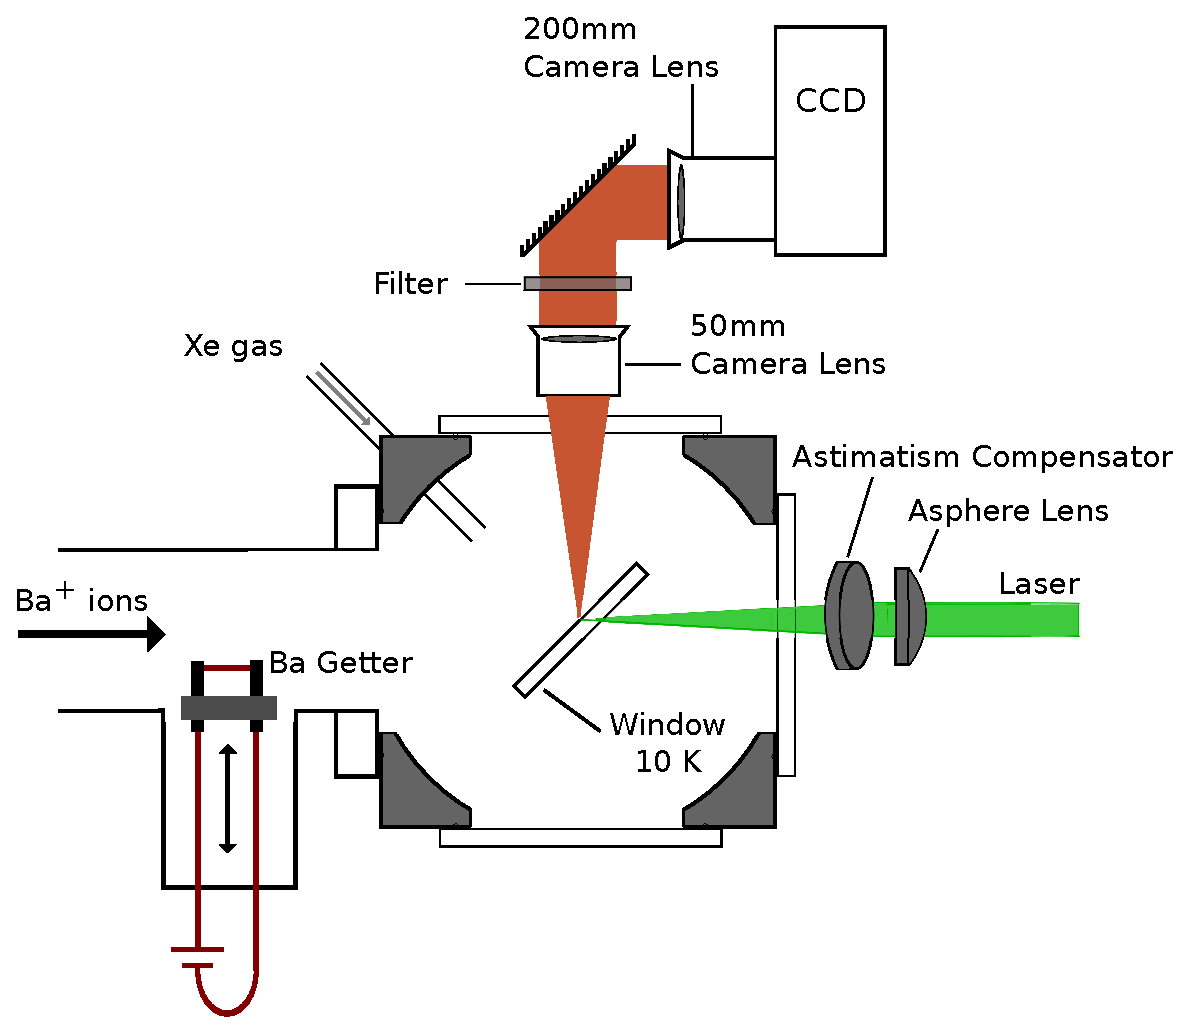
\includegraphics[width=0.5\textwidth]{figures/cryo_inkscape_chris_full.eps}
\caption{Experimental setup for depositing Ba/Ba\textsuperscript{+} in sXe matrices, and for excitation and imaging of the deposited atoms/ions.}
\label{fig:apparatus}
\end{figure}

Deposits are made on a cold sapphire window tilted at 40-45$^{\circ}$.  To create a sample, Xe gas is directed toward the window using a leak valve. The Xe gas freezes on the window and forms a sXe matrix with a thickness of around half a micron.  This is initiated a few seconds prior to the Ba deposit, continues during the Ba deposit, and is turned off a few seconds after the Ba deposit.

In this work, deposits are made with the sapphire window at around 50~K, partly to reduce hydrogen content in the matrix, as hydrogen condenses well below 50~K in vacuum \cite{Mong2015}.  The window is then cooled to 11~K for observation.  Deposits made at 50~K exhibit higher 619-nm signal than those made at 11~K.  Xe deposition at around 30~nm/s also exhibit higher 619-nm signal, as compared to lower leak rates, while not being so high as to produce a frosty Xe matrix.  An experiment cycle consists of a deposit at 50 K, a fluorescence observation at 11 K, and then the deposit is evaporated by heating the window to 100 K.  Many deposits are made in a day with varying numbers of ions deposited, as well as periodic Xe-only deposits to establish the background.
%, likely due to a higher population of 619-nm matrix sites

The excitation laser, a Coherent 599 cw dye laser with Rhodamine 6G dye pumped by the 514-nm line of a Lexel 3500 argon ion laser, enters from the back side of the window.  Ba fluorescence light is collected and collimated by a 50~mm Nikon camera lens.  A band-pass filter with FWHM of 20~nm passes just the 619-nm fluorescence peak.  A 200~mm Nikon camera lens then focuses the image onto a liquid nitrogen cooled CCD, resulting in an image of $4 \times$ magnification.  Each of the 20$\times$20 $\mu$m pixels of the CCD represents approximately a 5$\times$5 $\mu$m area on the sXe sample.

For a given laser intensity, the smallest focus possible is desired for optimal signal-to-noise from single atoms.  To achieve this, an aspherical lens of 7.9~cm focal length \cite{asphere} is used to minimize spherical aberration, and a fused silica optical flat of 1~cm thickness is placed at 6$^{\circ}$ after the lens in order to compensate for astigmatism caused by the tilted sapphire window (Fig. \ref{fig:apparatus}).  Vibrations of the sapphire relative to the excitation laser must also be considered, as this will increase the area of laser exposure, and thus the number a Ba atoms illuminated.  Vibration compensation is discussed in Section \ref{subsec:vibes}. %  To reduce the exposed region, a shutter, placed the laser path, is synchronized with the signal from an accelerometer on the outside of the cryostat, such that the laser exposure is reduced to one lobe of the vibration.  Measurements of these vibrations and the effectiveness of the synchronized shutter are discussed in Section \ref{subsec:vibes}.
%was in 1h:  Though the number of Ba atoms instantaneously exposed is independent of vibrations, reducing the effectively exposed area is desirable in clarifying the definition of the laser region.

\subsection{Vibration Compensation}
\label{subsec:vibes}

\begin{figure}
%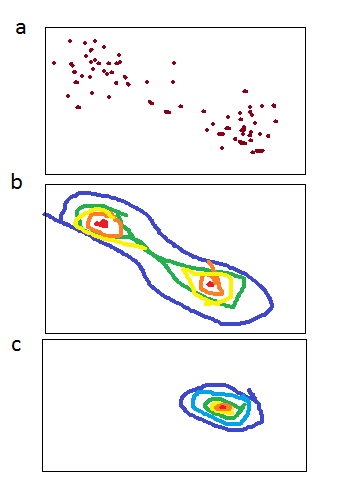
\includegraphics[width=0.3\textwidth]{figures/vibes_placeholder.png}
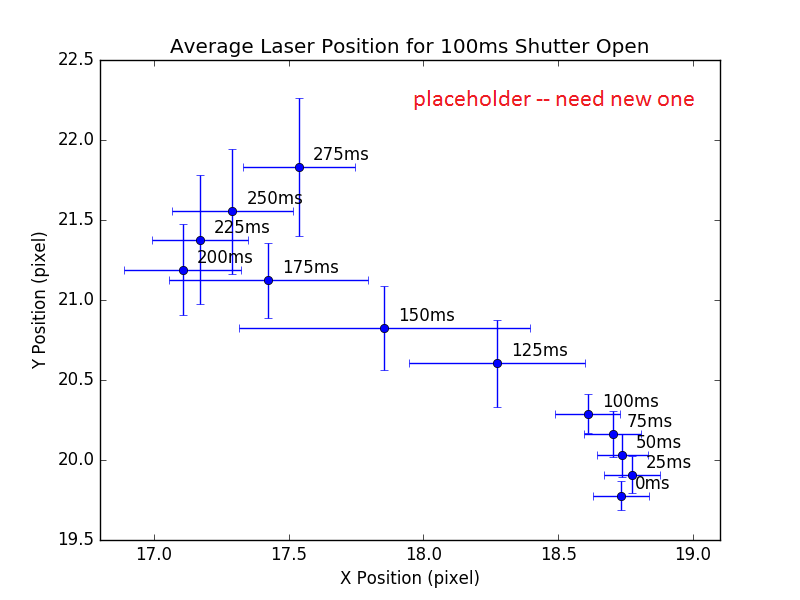
\includegraphics[width=0.5\textwidth]{figures/vibes_avepos_placeholder_100msShutter.png}
\caption{\color{gray}Using this?  Change labels to add the 40ms of natural delay, make axes microns}
\label{fig:vibes}
\end{figure}

%\begin{figure}
%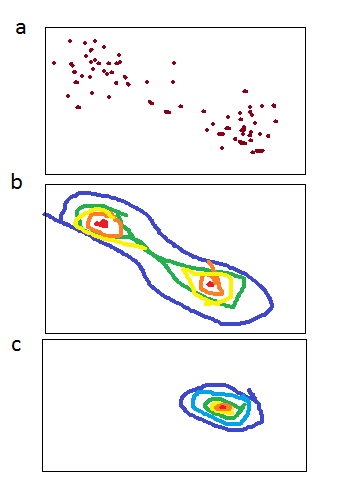
\includegraphics[width=0.3\textwidth]{figures/vibes_placeholder.png}
%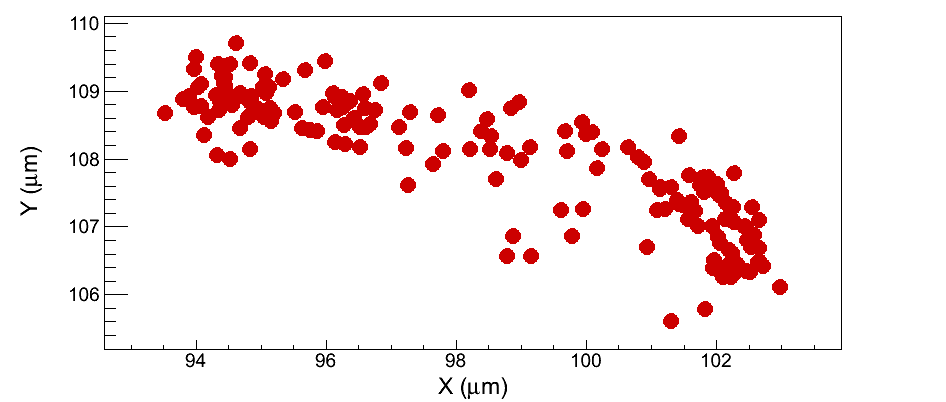
\includegraphics[width=0.5\textwidth]{figures/vibes_a.png}
%~
%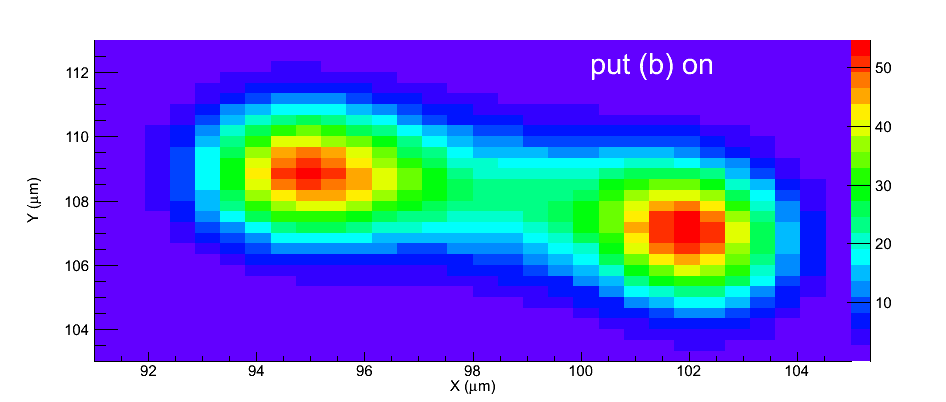
\includegraphics[width=0.5\textwidth]{figures/vibes_b.png}
%~
%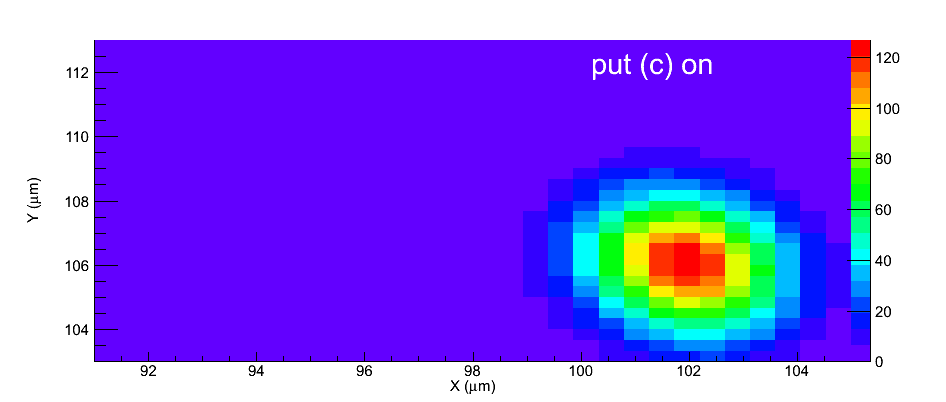
\includegraphics[width=0.5\textwidth]{figures/vibes_c.png}
%\caption{\emph{Explain in caption how (b) and (c) are 1-amplitude gaus sums of [x] points or whatever they actually are...\textbf{and magnitudes are different, I guess there are more points in c?} Get axis labels/titles same size.}}
%\label{fig:vibes}
%\end{figure}
%  (e) should really be the smeared one... maybe we don't need (d) and (e)?

Vibrations of the sapphire window relative to the excitation laser were studied by observing movement of a ``dust spot" on the sapphire window relative to the image of the laser on time scales of 100 ms, with the band-pass filter removed.  Dust spots are highly scattering objects which are fixed to the sapphire window.  They can be avoided when imaging Ba deposits, however they are useful in studies like this.

The major vibration is caused by the cryostat He pump, which pulses with a frequency of about 2.5~Hz.  To isolate the laser exposure to a smaller segment of this vibration region, a shutter, placed in the laser path, is synchronized with the signal from an accelerometer on the outside of the cryostat.  The shutter is triggered by the accelerometer with a specified delay time and open time.  The relative position between the sapphire window and the laser, averaged over about 60 points, is shown in Fig. \ref{fig:vibes} for several different delay times.  It was determined that about 40~ms of delay time and 200~ms open time are optimal, resulting in laser exposure localized to the lower right region. %on only one of the vibration lobes, as shown in Fig. \ref{fig:vibes}c.
%A typical vibration signal is shown in Fig. \ref{fig:vibeSig}.
% ...describe d and e?

%The relative position of a dust spot and the laser, determined with 2D Gaussian fits to the raw images, are plotted in Fig. \ref{fig:vibes}a, with a sampling of {\color{gray}200 50-}ms frames, each separated by {\color{gray}?} s of readout time.  2D Gaussian functions of width w$_{x}$ = 2.06~$\mu$m and w$_{y}$ = 2.66~$\mu$m, representing the minimum laser spot size, are overlain on each of these points and summed in Fig. \ref{fig:vibes}b, thus representing the total laser exposure on the sapphire window.  Sinusoidal vibration results in the majority of exposure occurring in two lobes.

% {\color{gray}It was determined that movement of the laser [negligible...]}

%\begin{figure}
%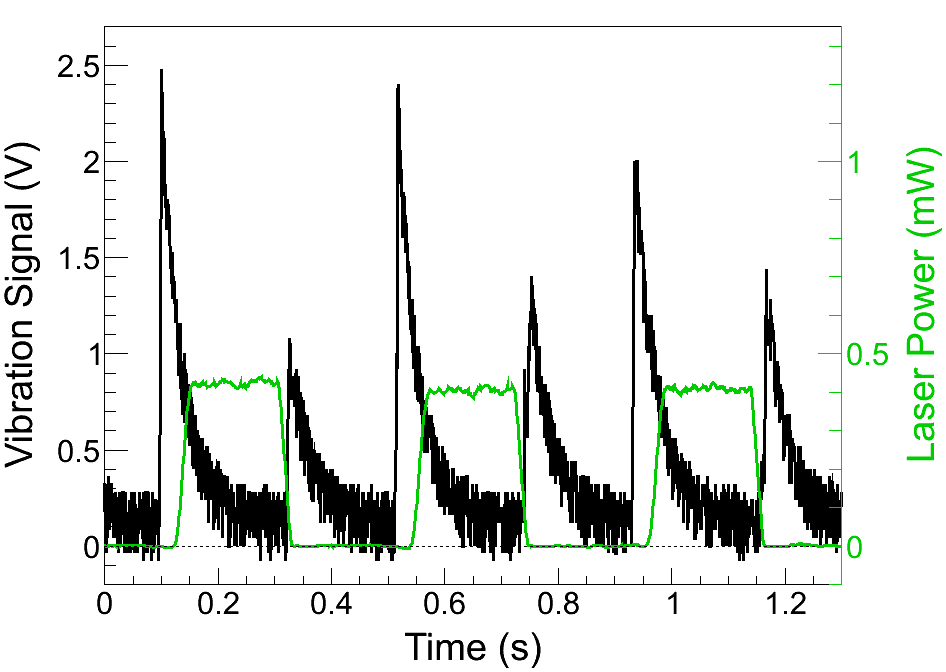
\includegraphics[width=0.5\textwidth]{figures/vibes_accelerometrSig.png}
%\caption{}
%\label{fig:vibeSig}
%\end{figure}

\subsection{Backgrounds}
\label{sec:backgrounds}

%{\color{blue}These two paragraphs need to be combined and/or whatever, made relevant:

%Weak fluorescence of impurities (most likely sub-ppb of Cr\textsuperscript{3+}) in the sapphire window is seen along the laser's path as a weak vertical line.

A typical image made with a focused laser beam at 570~nm is shown in Fig. \ref{fig:image_example}.  Very low concentrations of Cr\textsuperscript{3+} in the sapphire bulk (sub-ppb level) produce a strong fluorescence at 693~nm, with a broad tail extending to the 610-630~nm region passed by the band-pass filter.  This produces the faintly visible line through the sapphire window.  The broad fluorescence is also assigned to Cr\textsuperscript{3+}, as its excitation spectrum is identical to that of the well-known lines around 693~nm.  Commercially available c-plane quality sapphire from Meller Optics and Rubicon Technologies has sufficiently low concentrations for detecting single Ba atoms.  At both ends of the vertical line, some background emission from the surfaces is observed.  At the front surface (at the top in the image), extra fluorescence is detected from a small number of Ba atoms within the focused laser.

\begin{figure}
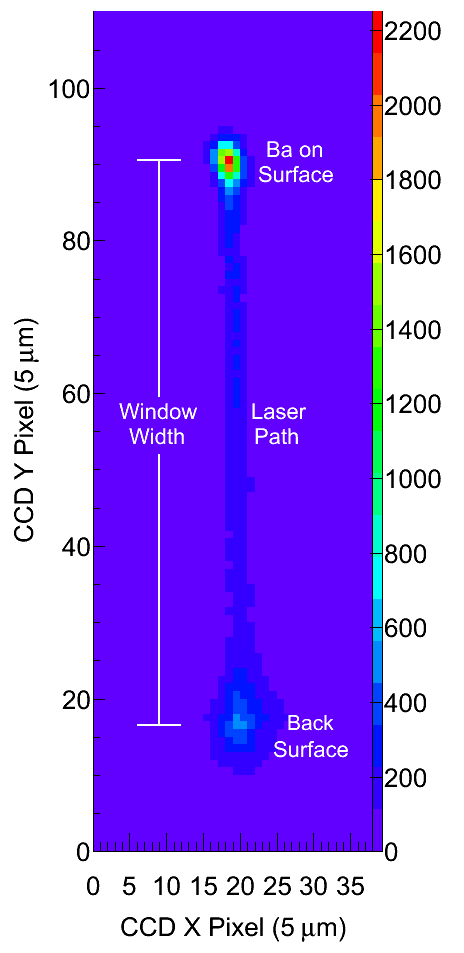
\includegraphics[width=0.3\textwidth]{figures/imageExamp_fromthesis.png}
\caption{Example image of a Ba\textsuperscript{+} deposit in sXe on a tilted c-plane sapphire window of 0.5~mm thickness.} % excited by a focused 570-nm laser, using a 620-nm fluorescence band-pass filter.}
\label{fig:image_example}
\end{figure}

The background emission from the sapphire surface is the main challenge for single Ba imaging.  It has been found that this background can be reduced significantly and semi-permanently by bleaching.  A variety of wavelengths have been used for bleaching, including 514.5~nm, 532~nm, 570-572~nm, and 580.5~nm.  The deposits discussed in Section \ref{sec:results} were done after {\color{gray}\textbf{...[the following is sort of a place-holder.  Either (A) we replace it with what is true for the data shown here (8-7 I think), or if we put newer data here, (B) input relevant numbers here]...} an overnight raster scan of a 20~mW 532~nm laser, focused to around w$_{0}$ = 10~$\mu$m, in a {\color{gray}?$\times$?}~position grid, with {\color{gray}?}~$\mu$m grid spacing and {\color{gray}?}~s at each position, in a repeating scan.  This was done with the sapphire window at 105~K.  As seen in Fig. [scanned im. of hole], this reduced the surface background over a region of about {\color{gray}?$\times$?}~$\mu$m to a level of ???.  This area is large enough to accommodate typical drift of about 1 pixel (5~$\mu$m) of the laser beam throughout a day.}

%{\color{gray}To minimize the surface background, the window is exposed to the laser until the background reaches a negligible value, prior to a series of measurements.}  {\color{red}The set of deposits used for Fig. \ref{fig:ctsVsIons} was done after about an hour of pre-exposure of the sapphire window to the focused laser.}  \emph{\color{gray}This will be different with the new, ``ultimate" data set, and maybe there will be more discussion here on the bleaching scan, possibly showing scanned images of the bleached region.  Bill:  \textbf{Probably need to rewrite this with more details and possibly an image if new data with scanned bleaching at 100K is used.}}
%, though its bleaching rate is different from that of the 619-nm Ba emission
%, also caused by laser excitation.  This is more of a nuisance, as it not as easily distinguished from the Ba in an image

%Note that backgrounds due to impurities are not expected in the high-purity lXe environment of nEXO.

%\emph{\color{gray}Do we want a bleaching section?}

\subsection{Identification of 619-nm Peak as Ba in sXe}

Spectra of neutral Ba deposits made with the Ba getter source are compared to spectra of a Ba\textsuperscript{+} deposit in Fig. \ref{fig:ion_getter_ar}.  Identical spectra are observed using the different sources under similar deposit conditions.  This confirms that the images measured are of Ba atoms resulting from neutralization of the incident Ba\textsuperscript{+} ions.  Another peak at 670~nm which is mentioned in \cite{Mong2015} is also attributed to Ba.  No similar fluorescence is observed from deposits of Ar\textsuperscript{+} ions in sXe (Fig. \ref{fig:ion_getter_ar}) at 2000~eV under the same conditions.  This rules out matrix damage, e.g. fluorescent color centers, as the source of the 619-nm peak.  The linearity of the fluorescence signal vs. number og Ba\textsuperscript{+} ions at low flux supports an assignment to atomic Ba, as opposed to molecular Ba$_{2}$
%Observing Ba in the 619-nm matrix site at the low-energy (thermal) deposit from the getter is also good news for the prospect of grabbing Ba/Ba\textsuperscript{+} on a probe out of lXe.
%\emph{\color{gray}, though fluorescence vs. ions deposited has not been studied for this peak}

\begin{figure}
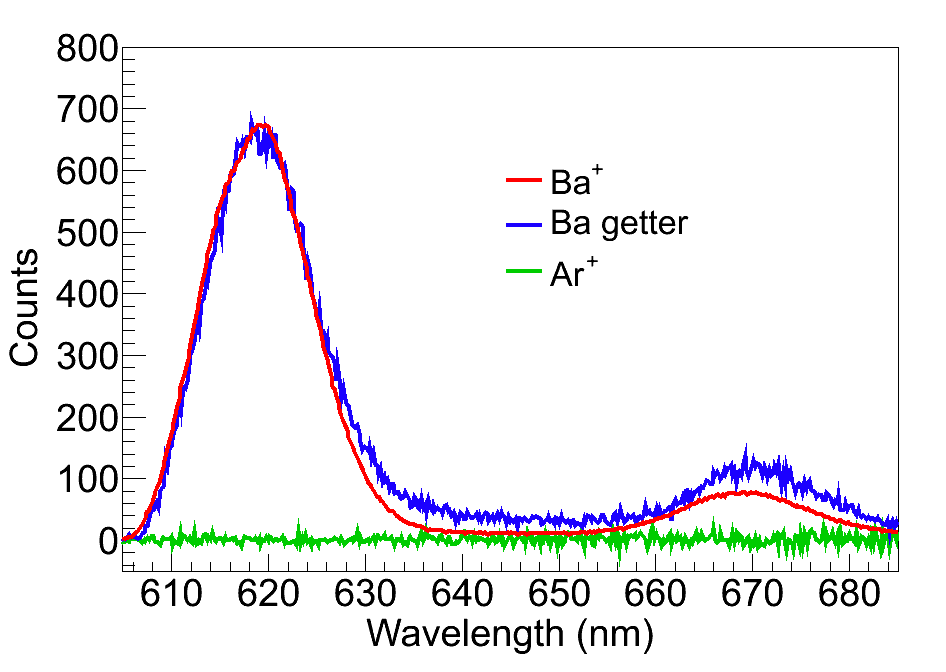
\includegraphics[width=0.48\textwidth]{figures/getter_fromthesis_Ar_vs_Ba.png}
\caption{Observation of deposits from three different sources in sXe.  Curves are scaled due to different deposit sizes.}
\label{fig:ion_getter_ar}
\end{figure}
%getter_ion_Ar_calibrated

%Ion currents of 30~nA and Xe deposition rates of 50~nm/s result in a Xe:Ba ratio of around 10\textsuperscript{4}:1.  This is 10~x higher than the recommended host:guest ratio [ref that old paper ... well, Brian's thesis says itand it's probably in that book you have to buy] for isolating Ba atoms in the matrix.

%{\color{red}I'm having trouble re-producing this, so maybe we leave it out:  }{\color{gray}Finally, a measurement of the Ba\textsuperscript{+} beam velocity confirms a mass of $137(?) \pm ?$, ruling out any contribution of barium oxide }(But probably not BaHx\textsuperscript{+}){{\color{gray}in the beam.  This is possible by knowing (a) the energy of the ions (2000~eV), (b) the time between the signals in a set of induction plates and the Faraday cup as well as the distance between the two, and (c) the timing of those signals for a pulse of Ar\textsuperscript{+} at the same energy, whose mass we know.  }

%{\color{gray}[Is there a statement we can make about molecules with lighter (O2, N2, H2, ...) being likely to show us mode peaks?]}


%\subsection{Temperature Dependence}

%Bad:  The temperature dependence of the 619-nm fluorescence is shown in Fig. \ref{fig:anneal} through three annealing cycles of a deposit made at 11~K.  The first anneal results in an overall larger signal upon returning to 11~K.  In anneal 2, lower fluorescence is observed at higher temperature, but essentially no signal is lost after returning to 11~K.  Anneal 3, to higher temperature of 48~K, does result in loss of overall signal.  {\color{red}[\textbf{If this is confusing or not relevant to the paper, we should leave out the whole subsection of temp. dependence, but not much was said about the 619 peak in the spec. paper.  I meant for this to show the fact that we need to be this cold to observe the peak in vacuum}]}  This temperature dependence of the fluorescence means that the probe in nEXO may need to be moved to a location out of the lXe where it can be cooled to 10 - 15~K.

%\begin{figure}
%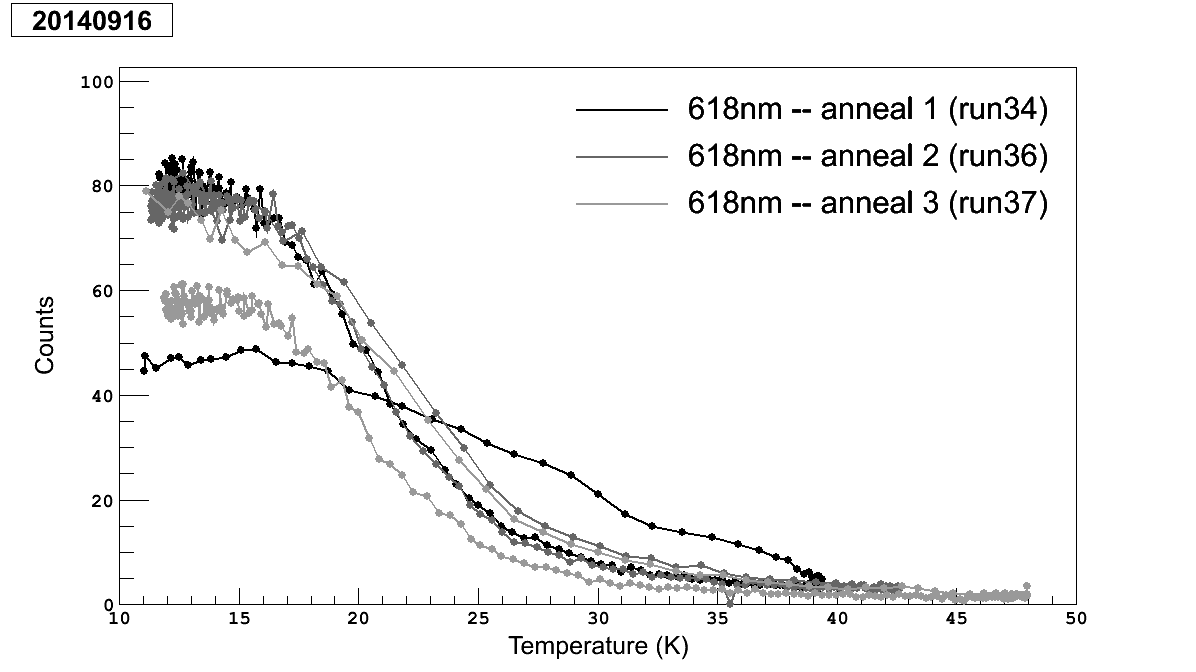
\includegraphics[width=0.5\textwidth]{figures/anneal_green_20140916_runs34-37_bg64_v12_618nm.png}
%\caption{Observing 619-nm peak through annealing process of a deposit made at 11~K.  {\color{red}[Will need nicer plot if we show this]}}
%\label{fig:anneal}
%\end{figure}

%\section{Discussion}

%It is worth noting that the initially lower amplitude of the 619-nm peak, vs. the peaks around 590~nm, does not imply anything about their relative populations.  Different matrix sites can have very different effects on electron transition rates, and fluorescence efficiencies can be quite different.  In fact, the fluorescence efficiency of the 619-nm site is measured to be {\color{red}$1 \times 10^{-5}$}, calculated using the cross section of Ba in sXe reported in \cite{Mong2015}.

\section{Results}
\label{sec:results}

%{\color{gray}[The excitation spectrum for the 619-nm peak is shown in Fig. \ref{fig:excitspec}.  An excitation wavelength of 570~nm is used.]}

%\begin{figure}
%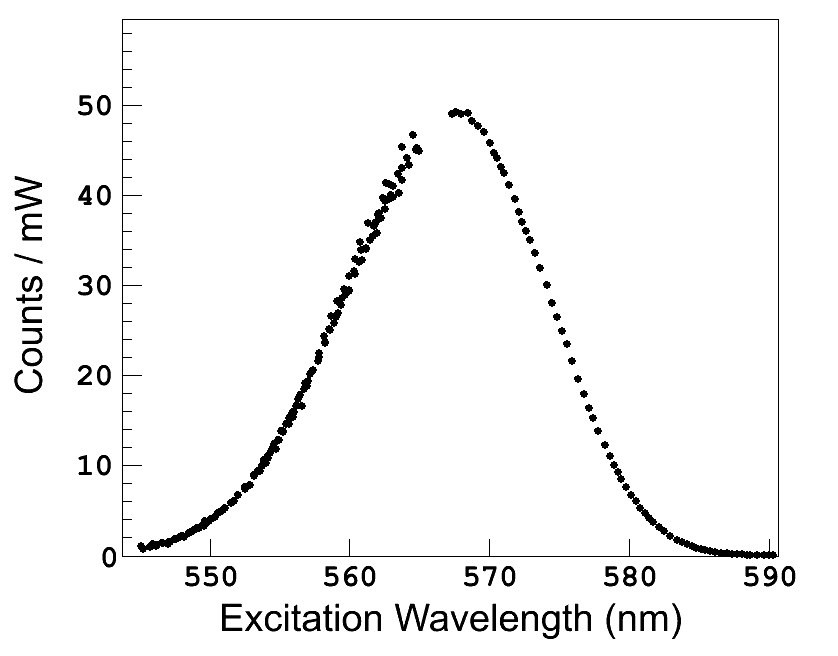
\includegraphics[width=0.48\textwidth]{figures/excitspec.png}
%\caption{Excitation spectrum for the 619-nm emission peak.  The discontinuity is due to use of different laser dyes, Rhodamine 110 and Rhodamine 6G.  The vertical scale is fluorescence normalized to laser power with an arbitrary scaling.}
%\label{fig:excitspec}
%\end{figure}

%moved this to the Backgrounds section since the image is refered to there:
%A typical image made with a focused laser beam at 570~nm is shown in Fig. \ref{fig:image_example}.  Weak fluorescence of impurities (most likely sub-ppb of Cr\textsuperscript{3+}) in the sapphire window is seen along the laser's path as a weak vertical line.  At both ends, some background emission from the surfaces is observed.  At the front surface (at the top in the image), extra fluorescence is detected from a small number of Ba atoms within the focused laser.

The number of Ba\textsuperscript{+} ions deposited within the 1/e radius of the laser beam gives a rough upper limit to the number of Ba atoms responsible for the observed signal.  For typical ion pulses of 13~fC/pulse and focused laser 1/e\textsuperscript{2} radii of w$_{0x}$ = 2.06~$\mu$m and w$_{0y}$ = 2.66~$\mu$m, this results in about 0.035 Ba\textsuperscript{+} ions/pulse in the 1/e intensity laser region.  The signal in Fig. \ref{fig:image_example} corresponds to a deposit of about 10 Ba\textsuperscript{+} ions into the laser region, and is therefore roughly due to $\leq 10$ Ba atoms.  Deposits of $\leq 39$, $\leq 3$, and $\leq 1$ Ba atoms are shown in Fig. \ref{fig:XeBaXe}a,b,c, respectively, with Xe-only deposits made before and after each Ba\textsuperscript{+} deposit.  The background level is determined by averaging the summed CCD counts in the focused laser region from the two surrounding Xe-only deposits for each Ba\textsuperscript{+} deposit.  The Ba fluorescence counts are determined by subtracting this background from the total counts in the same laser beam region in the image of the Ba\textsuperscript{+} deposit.  A significant finding is that {\color{gray}after a large deposit of $\leq 6.1 \times 10^4$ Ba atoms, the background in the next Xe-only deposit is the same as the Xe-only run before this deposit, as shown in Fig. \ref{fig:XeBaXeLarge}.\emph{[We need one with an actual preceding Xe run, and \textbf{need to look on lower scale at any BG change.} Also, \textbf{may want not quite so large a deposit} -- we actually don't know yet how large deposits affect it]}}  This is important for the implementation of this Ba tagging method in nEXO, so that false positives will not occur from previous Ba tags.

\begin{figure}
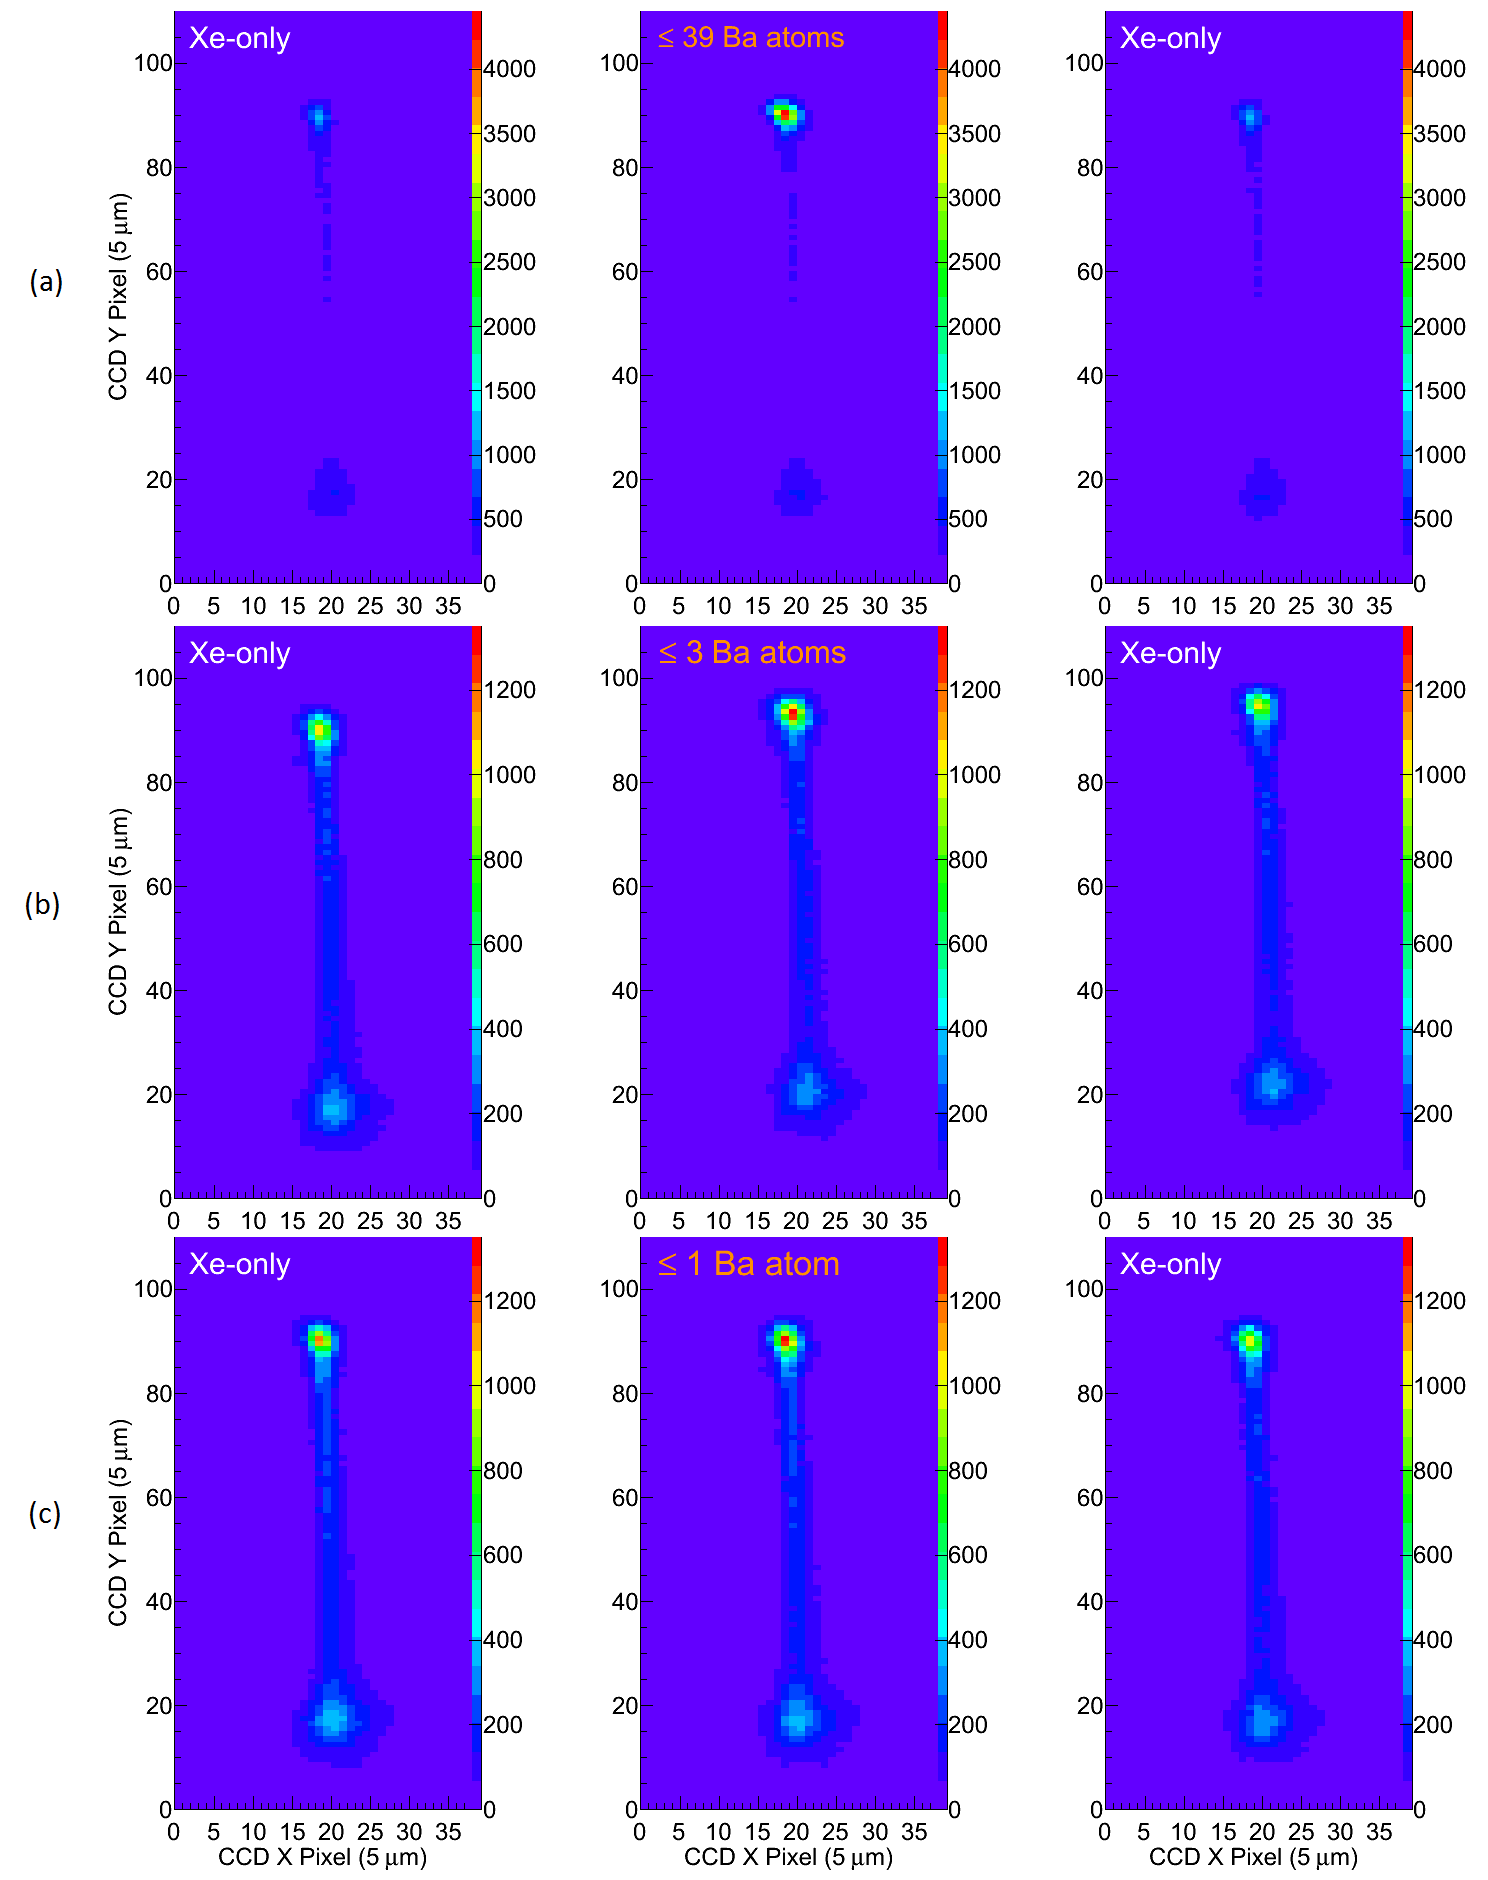
\includegraphics[width=0.5\textwidth]{figures/xebaxe_instantaneous_scrunched.png}
\caption{Images of Ba\textsuperscript{+} deposits yielding (a) $\leq 39$, (b) $\leq 3$, and (c) $\leq 1$ Ba atoms in the focused laser region, with Xe-only deposits done before and after each respective Ba\textsuperscript{+} deposit.  Exposures are 60~s with around 0.15~mW of 570-nm laser excitation.}
\label{fig:XeBaXe}
\end{figure}
%The samples were deposited at 50~K and observed at 11~K.  
%Xe-Ba-Xe_56-atom_71-73-74

\begin{figure}
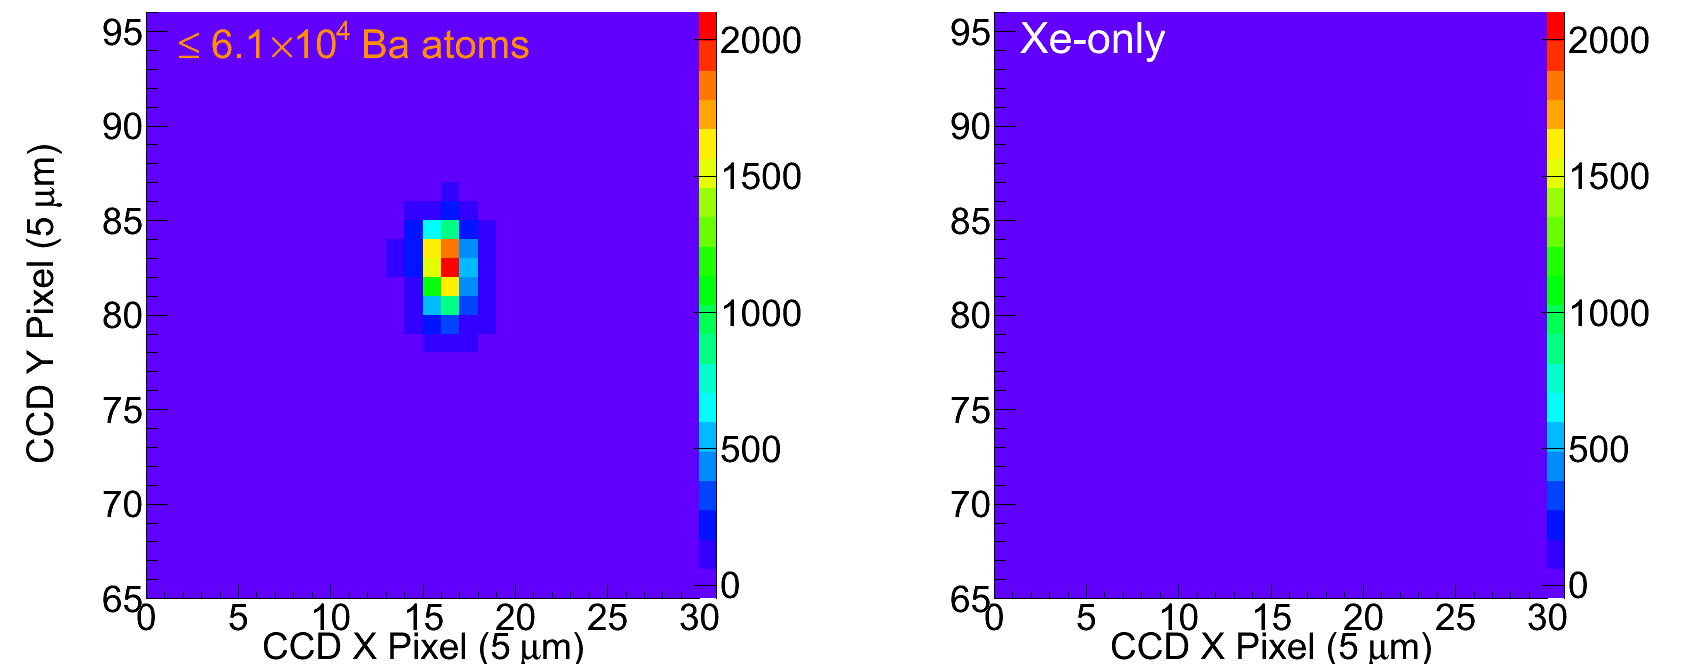
\includegraphics[width=0.5\textwidth]{figures/xebaxe_largest_instantaneous.png}
\caption{Image of a Ba\textsuperscript{+} deposit yielding $\leq 6.1 \times 10^4$ Ba atoms with its succeeding Xe-only deposit.  Exposures are 0.5~s with around 1.1~mW of 572-nm laser excitation.}
\label{fig:XeBaXeLarge}
\end{figure}
% The samples were deposited at 50~K and observed at 11~K.  

\begin{figure}
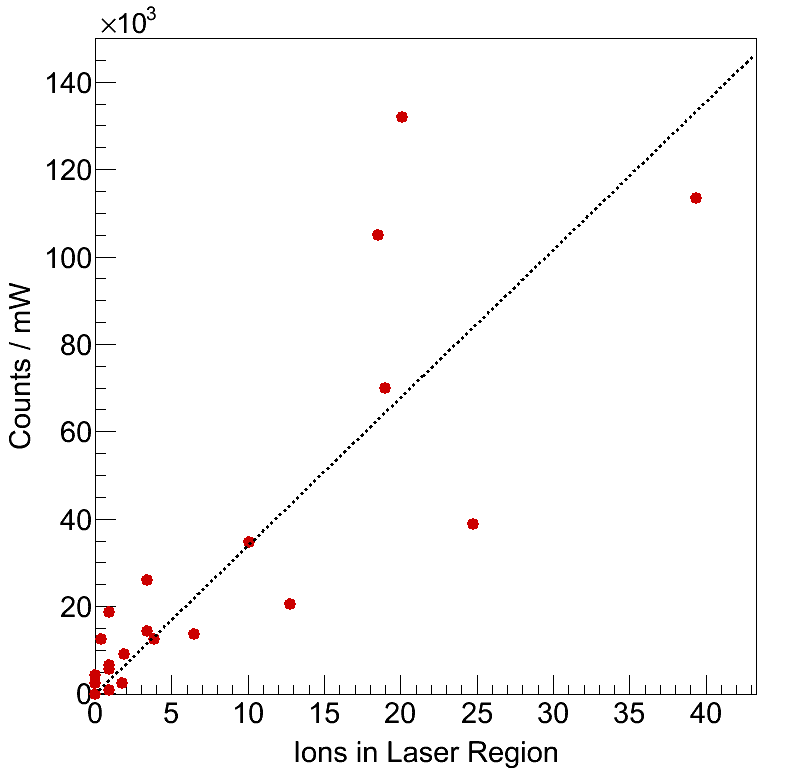
\includegraphics[width=0.48\textwidth]{figures/lin_just20150807_lin.png}
\caption{619-nm Ba fluorescence vs. number of ions deposited.  Exposures are 60~s with around 0.15~mW of 570-nm laser excitation.}
%say exposures are 'around' ? s for vibe-compensated ones since they're not always the same ... is it 572 nm in the newer stuff?
\label{fig:ctsVsIons}
\end{figure}
%  {\color{blue}\emph{Could use better ion beam consistency.}}

The Ba counts vs. Ba\textsuperscript{+} ions deposited in the laser region are plotted in Fig. \ref{fig:ctsVsIons}.  The summed CCD counts in the laser region in sXe of each image is linear with ions deposited.  The observed signal corresponds to $3400 \pm 360$~counts/mW per atom with around 0.15~mW of focused 572-nm laser excitation and around 60~s of laser exposure.  Counts are scaled by the integral of the power signal recorded by a power meter after the laser shutter.  Background-subtracted images of deposits near the linear trend line are shown in Fig. \ref{fig:train} corresponding to (a) $\leq 10$~atoms, (a) $\leq 3$~atoms, and (a) $\leq 1$~atom.  These represent the expected signal level, with a clear peak at the single-atom level.
%took this out because it makes it seem like there is variance in the plotted points as a result: Exact exposure times vary slightly according to the total open time of the vibration compensation shutter, as discussed in Section \ref{subsec:vibes}.

%{\color{gray}\textbf{Old paragraph, for the 8-7 plot:}  The Ba counts vs. Ba\textsuperscript{+} ions deposited in the laser region are plotted in Fig. \ref{fig:ctsVsIons}.  The summed CCD counts in the laser region in sXe of each image is linear with ions deposited{\color{gray}, albeit with significant scatter due to ion beam instabilities in this run}.  The observed signal corresponds to $3400 \pm 360$~counts/mW per atom with around {\color{gray}0.15~mW} of focused 570-nm laser excitation, and 60-s CCD exposures.  Counts are scaled by laser power to account for small variations in laser power.  Background-subtracted images of deposits near the linear trend line are shown in Fig. \ref{fig:train} corresponding to (a) $\leq 10$~atoms, (a) $\leq 3$~atoms, and (a) $\leq 1$~atom.  These represent the expected signal level, with a clear peak at the single-atom level.}
%For each point, the counts from a nearby Xe-only run have been subtracted.

%\emph{\color{gray}Maybe show the train thing instead? and re-word (``in the laser beam" and ``one ion depositied?"): A subtracted image of a deposit corresponding to a single Ba atom is shown in Fig. \ref{fig:lego}.  \st{A solitary peak is observed from the Ba in the laser region.}(``need comment on on clear peak")}

%\begin{figure}[h!tb]
%	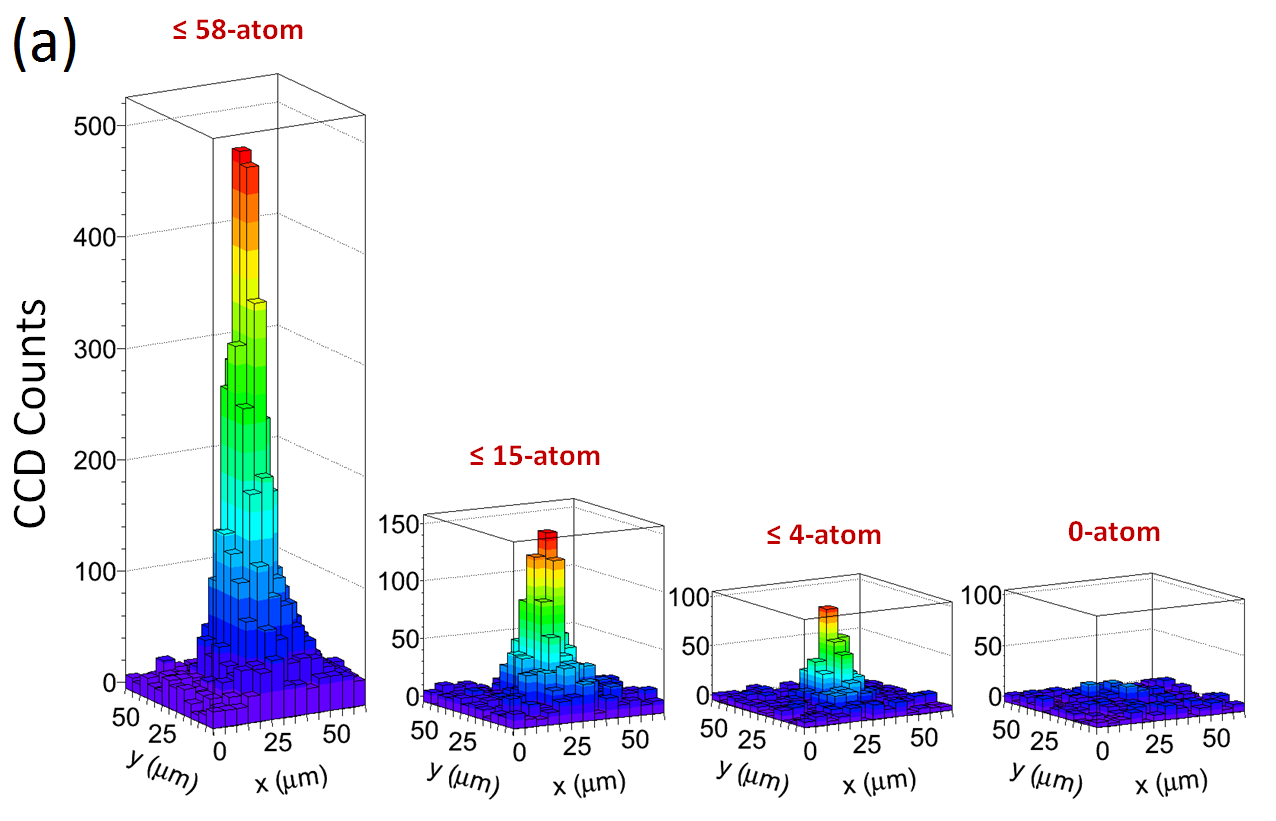
\includegraphics[width=0.45\textwidth]{figures/lego_varying.png}
%	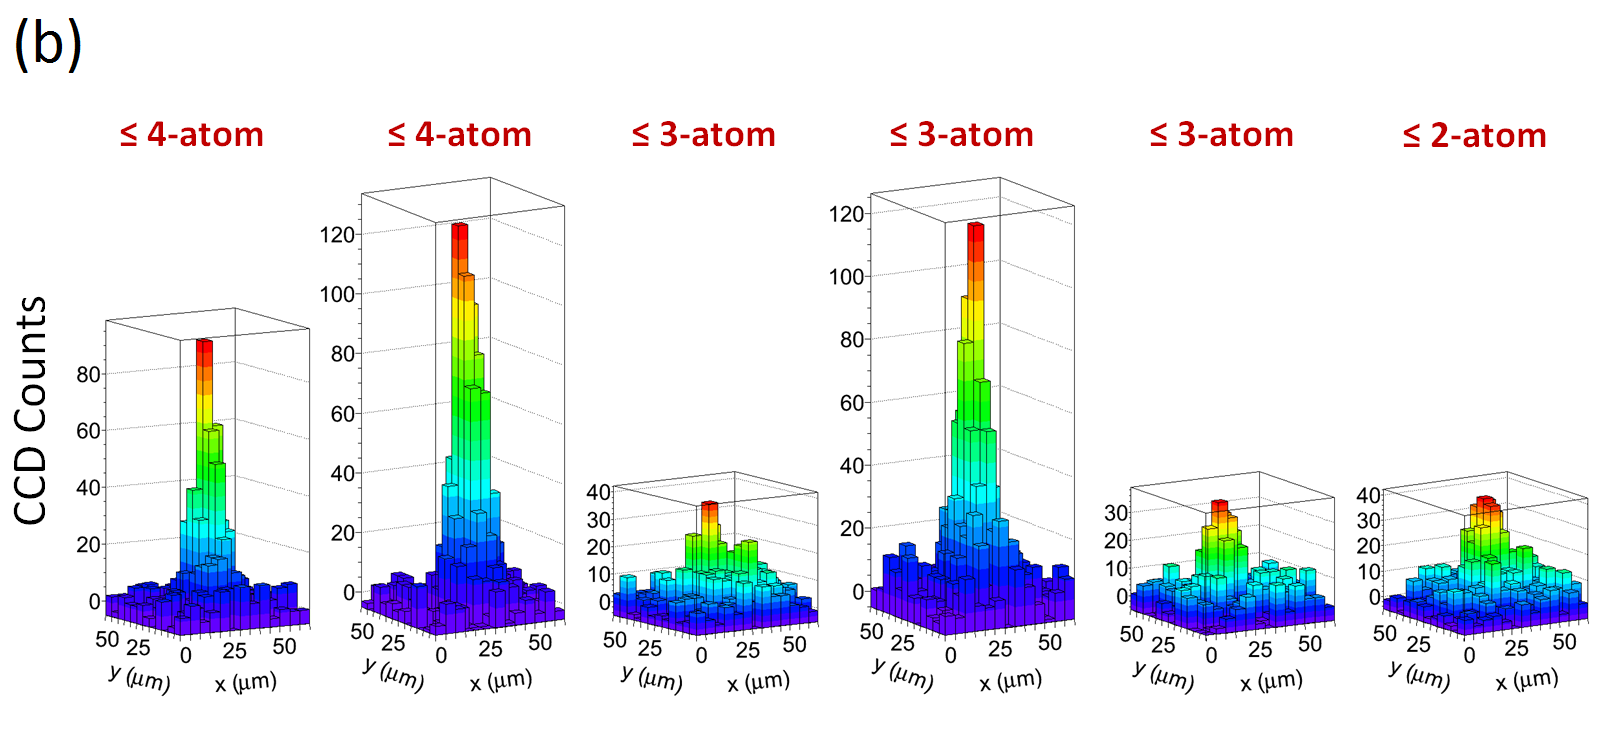
\includegraphics[width=0.45\textwidth]{figures/lego_statistical.png}
%	\caption{Images of small numbers of Ba atoms in a focused laser beam.  {\color{red}Maybe need to specify conditions.}}
%	\label{fig:lego}
%\end{figure}

\begin{figure}
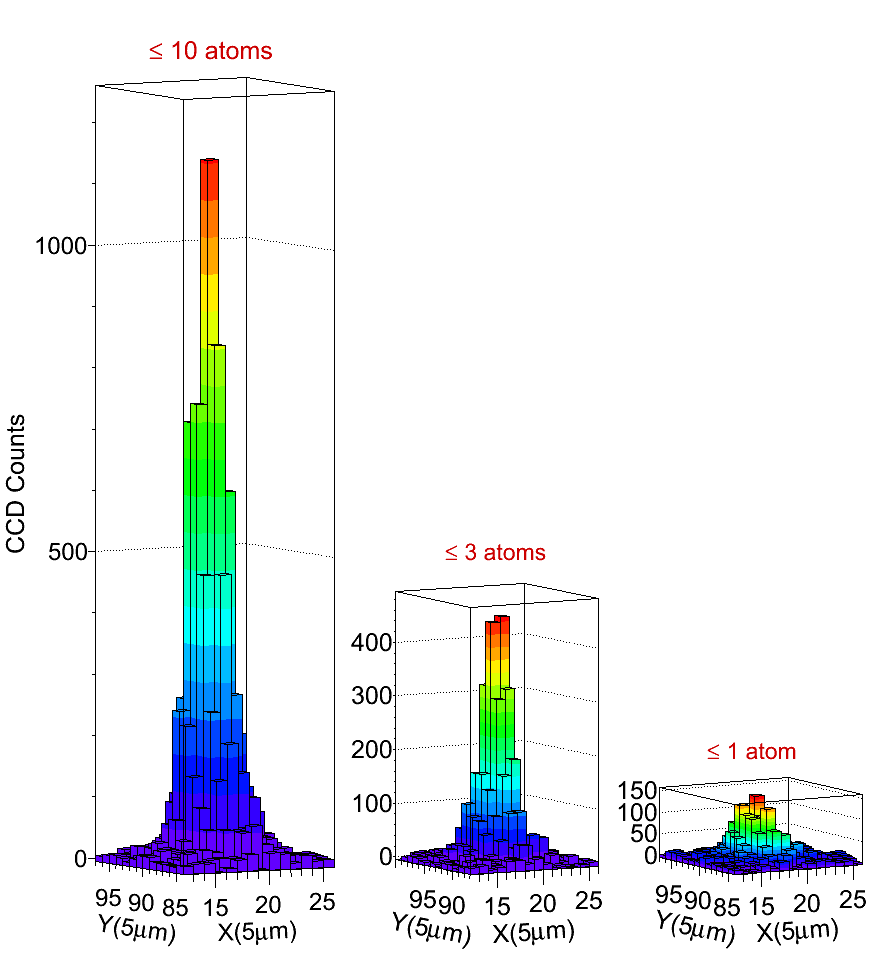
\includegraphics[width=0.48\textwidth]{figures/lego_train_fromthesis.png}
\caption{Subtracted images of 619-nm fluorescence in the focused laser region for runs near the linear trend line in signal vs. ions deposited.  Exposures are 60~s with around 0.15~mW of 570-nm laser excitation.}
\label{fig:train}
\end{figure}
%The samples were deposited at 50~K and observed at 11~K. 
%Image of a single Ba atom (on average) in a focused w = 2.1~$\mu$m laser beam, with 60~s exposure of 0.18~mW laser power.

%\begin{figure}
%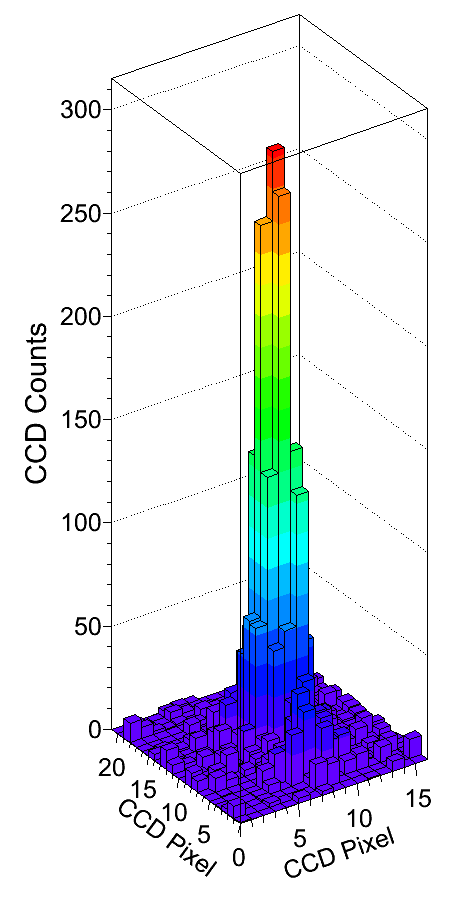
\includegraphics[width=0.48\textwidth]{figures/lego_near-line_1-atom.png}
%\caption{Image of a single Ba atom (on average) in a focused w = 2.1~$\mu$m laser beam, with 60~s exposure of 0.18~mW laser power.}
%\label{fig:lego}
%\end{figure}

A Gaussian fit to the images gives a 1/e$^{2}$ radius of 12~$\mu$m, which is much larger than the average laser beam radius of w = 2.4~$\mu$m.  Aberrations and vibrations in the collection optics and imperfections in the surface of the sXe layer could contribute to blurring of the image.

%{\color{red}\textbf{[This part needs to be rewritten with new results on vibration and bleaching -- Vibration will be described and then procedure for eliminating vibration included somewhere in this paper.  You will have to figure out where and how to fit it in]}A Gaussian fit to the images gives a 1/e$^{2}$ radius of 12~$\mu$m, which is much larger than the average laser beam radius of w = 2.4~$\mu$m} {\color{gray}(that part is still true, but it may not meld into the next discussion as well...)}.  {\color{red}Aberrations and vibrations in the collection optics and imperfections in the surface of the sXe layer could contribute to blurring of the image.  Relative motion of the laser and the window could also lead to exposure of more Ba atoms than calculated above.  The latter effect has been checked by observing images of the focused laser relative to a reference point on the sapphire window on time frames down to 50~ms.  Sinusoidal vibrations were observed on the order of 12~$\mu$m in x and 5~$\mu$m in y, due to cryostat vibrations, which corresponds to a total coverage of about 4.7 times the laser region.  However, the signal at a given time still comes from an area the size of the laser region.  Thus, the signals observed correspond to the above-quoted instantaneous number of Ba atoms illuminated according to the laser spot size, though the total number of atoms illuminated is about 4.7 times larger.}
%The latter effect has been checked by measuring intensity variations of the laser beam and its reflection from the window when cut 50\% by a razor blade.  {\color{blue}Maximum vibrations observed were on the order of ?~$\mu$m and ?~$\mu$m peak-peak for the laser and reflection, respectively}.

%\subsection{Scanned Images}

%\emph{\color{blue}Put scanned image of single atoms here.}

\section{Conclusions}

The 619-nm emission peak observed in deposits of Ba\textsuperscript{+} and Ba in sXe is attributed to neutral Ba in a stable and relatively abundant matrix site.
%An excitation spectrum and temperature dependence of the fluorescence are reported.
Images of 619-nm fluorescence in a focused laser region from Ba atoms are achieved down to the single-atom level.  Successful detection of Ba atoms in sXe at this level is a significant step toward Ba tagging in nEXO. 

\section*{Acknowledgements}

This material is based upon work supported by the National Science Foundation under Grant Nunber PHY-1132428 and the U.S. Department of Energy, Office of Science, Office of High Energy Physics \textbf{\textcolor{red}{under Award Number DE-FG02-03ER41255. (check that)}}
%Shon Cook and Brian Mong for pioneering work and primary authorship in \cite{Mong2015}.  

%\bibliography{references10}
\begin{thebibliography}{00}
 \bibitem{ReviewNuMass} K.A. Olive \emph{et al.} (Particle Data Group), \emph{Chin. Phys. C} \textbf{38}, 090001 (2014) (http://pdg.lbl.gov).
 %``14. Neutrino Mass, Mixing, and Oscillations,"

%\bibitem{anticorr} E. Conti \emph{et al.}, \emph{Phys. Rev. B} \textbf{68}, 054201 (2003).

\bibitem{EXO200TwoNuLong} J. Albert \emph{et al.} (EXO-200 Collaboration), \emph{Phys. Rev. C} \textbf{89}, 015502 (2014).

\bibitem{EXO200ZeroNuNature} J. Albert \emph{et al.} (EXO-200 Collaboration), \emph{Nature} \textbf{510}, 229 (2014).

\bibitem{Moe1991} M. Moe, \emph{Phys. Rev. C} \textbf{44}, R931 (1991).

\bibitem{Mong2015} B. Mong \emph{ et al.}, \emph{Phys. Rev. A} \textbf{91}, 022505 (1954).

\bibitem{Twelker2014} K. Twelker \emph{ et al.}, \emph{Review of Scientific Instruments} \textbf{85}, 095114 (2014).

\bibitem{Brunner2015} T. Brunner \emph{ et al.}, \emph{International Journal of Mass Spectrometry} \textbf{379}, 110-120 (2015).

\bibitem{alphaion} J. Albert \emph{et al.} (EXO-200 Collaboration), \emph{Phys. Rev. C} \textbf{92}, 045504 (2015).

\bibitem{McCaffrey2016} B. Davis, J. McCaffrey, \emph{J. Chem. Phys.} \textbf{144}, 044308 (2016); doi: 10.1063/1.4940688

\bibitem{asphere} Thorlabs part ASL10142-A.
\end{thebibliography}

\end{document}